% =====================================================================
%  Appendix A — Application User Interface Screens
% =====================================================================
\chapter{Application User Interface Screens}
\label{app:screenshots}

This appendix presents the primary user interface screens of the Alcedo mobile application. Figure~\ref{fig:app_screens_appendix} displays the core screens.

\begin{figure}[htbp]
    \centering
    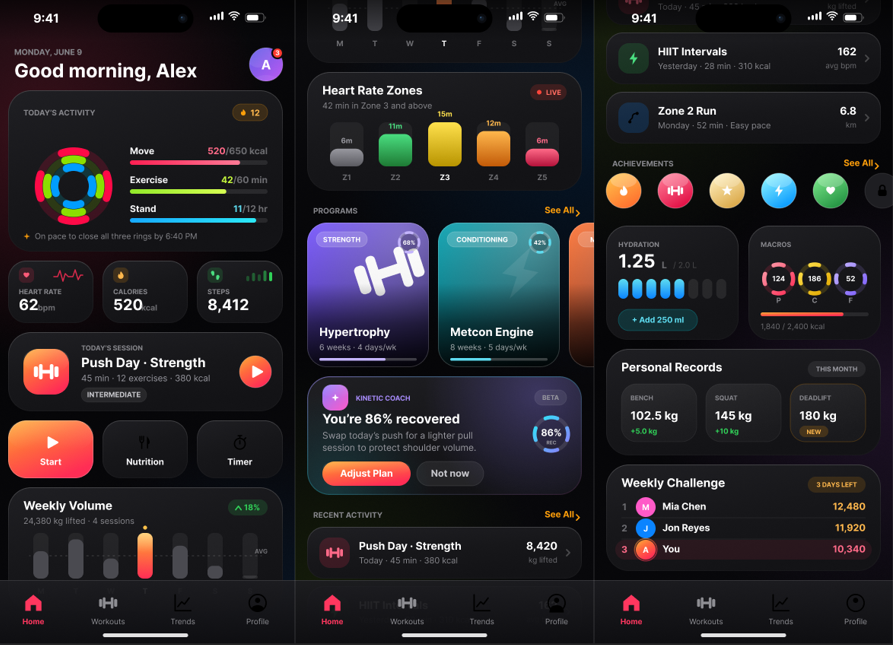
\includegraphics[width=5.5in]{screen.png}
    \caption{Alcedo Core Screens: Home Dashboard, Workout Execution, and Performance Analytics}
    \label{fig:app_screens_appendix}
\end{figure}

\section{Screen Overview}
The application encompasses twenty-four screens organized across five navigation tabs:

\subsection{Workout and Session Tracking}
\begin{itemize}
    \item \textbf{Home Dashboard:} Displays workout streaks, quick-start launcher, and assigned routine blueprints.
    \item \textbf{Live Workout Execution:} Set-by-set recording with weight/rep inputs, set-type toggles, rest timer, and exercise replacement.
    \item \textbf{Post-Workout Summary:} Session metrics including total tonnage, sets, reps, duration, and PR badges.
    \item \textbf{Workout Blueprint Editor:} Interface for constructing multi-week training programs.
    \item \textbf{Plan Diff-Save:} Side-by-side visual comparison when modifying existing routines.
\end{itemize}

\subsection{Exercise Library}
\begin{itemize}
    \item \textbf{Exercise Search:} Catalog search filtered by muscle group and equipment type.
    \item \textbf{Exercise Detail and History:} Execution guidance and historical weight/rep logs.
    \item \textbf{Custom Exercise Creator:} Registration of custom exercises with muscle and equipment classifications.
\end{itemize}

\subsection{History and Calendar}
\begin{itemize}
    \item \textbf{Training Calendar:} Monthly calendar with activity indicators and weekly workout list.
    \item \textbf{Session Editor:} Retroactive editing of completed workout logs.
\end{itemize}

\subsection{Performance Analytics}
\begin{itemize}
    \item \textbf{Trends Dashboard:} Training volume heatmaps and frequency graphs.
    \item \textbf{Progression Curves:} Estimated 1RM charts and muscle group load distribution.
\end{itemize}

\subsection{Settings and Configuration}
\begin{itemize}
    \item \textbf{Settings Hub:} User profile, display preferences, and diagnostics.
    \item \textbf{Theme Selection:} Light, Dark, and OLED mode switching with sound and unit toggles.
    \item \textbf{Backup and Restore:} Local JSON export/import and data sharing.
    \item \textbf{Backend Diagnostics:} Server URLs, token states, and feature probe results.
\end{itemize}
